
% This LaTeX was auto-generated from MATLAB code.
% To make changes, update the MATLAB code and republish this document.

\documentclass{article}
\usepackage{graphicx}
\usepackage{color}

\sloppy
\definecolor{lightgray}{gray}{0.5}
\setlength{\parindent}{0pt}

\begin{document}

    
    
\section*{Math 315 Lab 2}

\begin{par}
The following lab explores the basic routines for solving linear systems such as Gaussian Elimination with Partial Pivoting, Forward Subsitution for Lower Triangular systems, and Backward Substitution for Upper Triangular Systems. I will showcase that the row- and column-oriented routines are in fact row- and column-oriented from a theoretical and runtime perspective. Lastly, I will compare the runtimes of the GEPP algorithm with Matlab's backslash operator to solve a system.
\end{par} \vspace{1em}

\subsection*{Contents}

\begin{itemize}
\setlength{\itemsep}{-1ex}
   \item Forward Substitution for Lower-Triangular Systems
   \item Backward Substitution for Upper-Triangular Systems
   \item GEPP Routine
\end{itemize}


\subsection*{Forward Substitution for Lower-Triangular Systems}

\begin{par}
First, I will verify that my forward substitution routine for solving lower-triangular systems is accurate. I have coded both a row- and column-oriented routine and will also compare the time difference between the two. Since matlab is a column-oriented, I suspect that the column-oriented routine will be faster.
\end{par} \vspace{1em}
\begin{par}
Below is the code for row- and column-oriented Forward Substitution routines from the textbook.
\end{par} \vspace{1em}
\begin{verbatim}
disp(fileread('row_forward.m'))
\end{verbatim}

        \color{lightgray} \begin{verbatim}function x = row_forward(A, b)
    % Solve Ax=b, where A is an n-by-n lower triangular matrix,
    % using row-oriented forward substitution.
    if any(diag(A) == 0)
        error('Input matrix is singular')
    end
    n = length(b);
    x = zeros(n,1);
    for i = 1:n
        x(i) = (b(i) - A(i,1:i-1)*x(1:i-1)) / A(i,i);
    end
\end{verbatim} \color{black}
    \begin{verbatim}
disp(fileread('col_forward.m'))
\end{verbatim}

        \color{lightgray} \begin{verbatim}function x = col_forward(A, b)
    % Solve Ax=b, where A is an n-by-n lower triangular matrix,
    % using column-oriented forward substitution.
    if any(diag(A) == 0)
        error('Input matrix is singular')
    end
    n = length(b);
    x = zeros(n,1);
    
    for j = 1:n
        x(j) = b(j) / A(j,j);
        b(j+1:n) = b(j+1:n) - A(j+1:n,j)*x(j);
    end
\end{verbatim} \color{black}
    \begin{par}
Solving the system below, I show that the relative errors for both the row- and column-oriented routines for solving lower-triangular systems are super small.
\end{par} \vspace{1em}
\begin{verbatim}
A_L = [1 0 0; 2 1 0; 1 3 1];
b_L = [2; 5; 6];
x_exact_L = [2; 1; 1];

x_row_forward = row_forward(A_L, b_L);
row_forward_rel_err = ((norm(x_exact_L-x_row_forward)) / (norm(x_exact_L)));
fprintf("row-oriented forward substitution relative error: %f", ...
    row_forward_rel_err);

x_col_forward = col_forward(A_L, b_L);
col_forward_rel_err = ((norm(x_exact_L-x_col_forward)) / (norm(x_exact_L)));
fprintf("\ncolumn-oriented forward substitution relative error: %f", ...
    col_forward_rel_err);
\end{verbatim}

        \color{lightgray} \begin{verbatim}row-oriented forward substitution relative error: 0.000000
column-oriented forward substitution relative error: 0.000000\end{verbatim} \color{black}
    \begin{par}
To confirm my suspicions that the column-oriented routine for forward subsitution will run faster than the row-oriented routine for forward subsitution, I will run the two functions on 11 random and increasingly larger matrices to see how the runtimes compare.
\end{par} \vspace{1em}
\begin{verbatim}
n=(15000:100:16000);
row_forward_times=zeros(11,1);
col_forward_times=zeros(11,1);
for i=1:11
    A=tril(rand(n(i)));
    b=rand(n(i),1);
    tic;
    row_forward(A,b);
    row_forward_times(i)=toc;
    tic;
    col_forward(A,b);
    col_forward_times(i)=toc;
end

f1=figure(1);
clf(f1);
plot(n, row_forward_times, 'r')
hold on;
plot(n, col_forward_times, 'g')
legend({'row', 'col'}, 'FontSize', 12, 'Location', 'north')
xlabel('Matrix Size n')
ylabel('Time Used (s)')
title('Time Spent by Row- and Column-Oriented Forward Substitution')
hold off;
\end{verbatim}

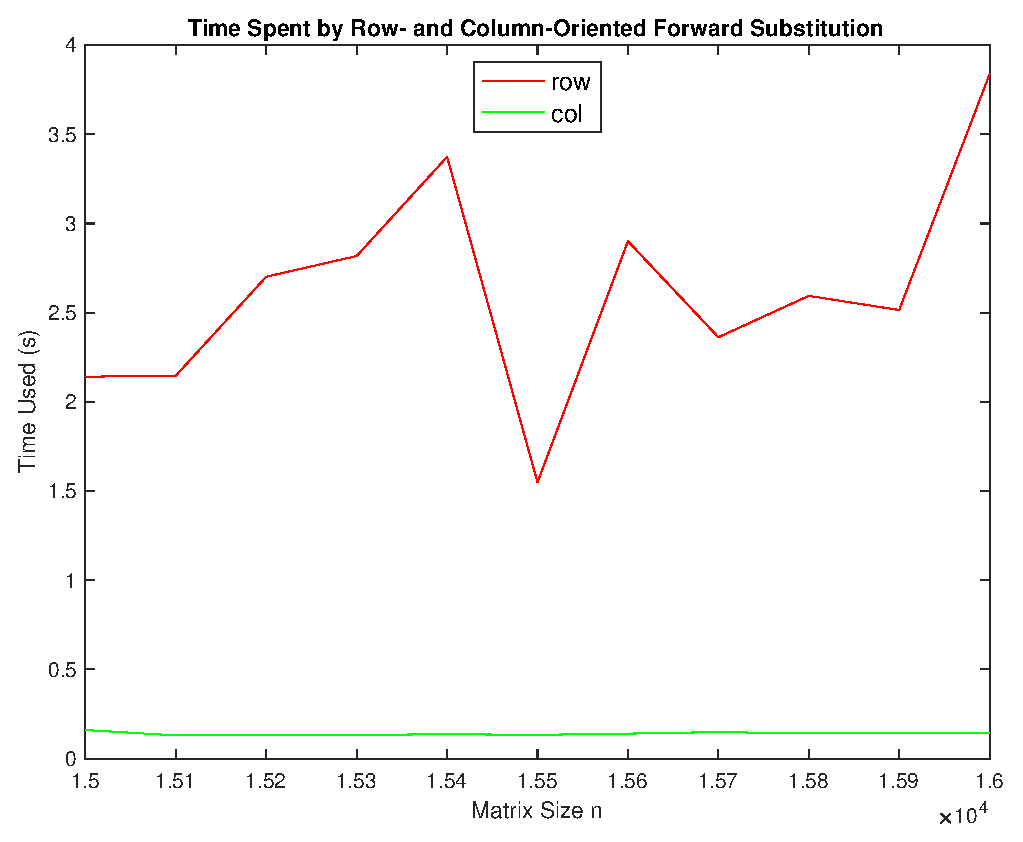
\includegraphics [width=4in]{Lab2_01.eps}


\subsection*{Backward Substitution for Upper-Triangular Systems}

\begin{par}
Next, I will verify that my backward subsitution routine for solving upper-triangular systems is accurate. I have also coded both a row- and column-oriented routines.
\end{par} \vspace{1em}
\begin{par}
Below are the row- and column-oriented routines for Backward Substitution. The row-oriented routine is in fact row-oriented because the outer for loop iterates through the rows and the inner for loop iterates through the columns. Therefore, the algorithm starts by solving the last row for the last x. Then it moves onto the second to last row and uses the x from before to solve that row. This then continues as each row is solved one after another using the previous rows findings.
\end{par} \vspace{1em}
\begin{par}
The column-oriented routine is in fact column-oriented because the out for loop iterates through the columns and the inner for loop iterates through the rows. This means that last term, which corresponds to the last column, is solved for every row as last entry of the column can produce the solutions to the last term. Then, the second to last column gets solved and so forth until the first column is solved.
\end{par} \vspace{1em}
\begin{par}
In fact, we can showcase this by looking at the difference in runtime of these two programs.
\end{par} \vspace{1em}
\begin{verbatim}
disp(fileread('row_forward.m'))
\end{verbatim}

        \color{lightgray} \begin{verbatim}function x = row_forward(A, b)
    % Solve Ax=b, where A is an n-by-n lower triangular matrix,
    % using row-oriented forward substitution.
    if any(diag(A) == 0)
        error('Input matrix is singular')
    end
    n = length(b);
    x = zeros(n,1);
    for i = 1:n
        x(i) = (b(i) - A(i,1:i-1)*x(1:i-1)) / A(i,i);
    end
\end{verbatim} \color{black}
    \begin{verbatim}
disp(fileread('col_forward.m'))
\end{verbatim}

        \color{lightgray} \begin{verbatim}function x = col_forward(A, b)
    % Solve Ax=b, where A is an n-by-n lower triangular matrix,
    % using column-oriented forward substitution.
    if any(diag(A) == 0)
        error('Input matrix is singular')
    end
    n = length(b);
    x = zeros(n,1);
    
    for j = 1:n
        x(j) = b(j) / A(j,j);
        b(j+1:n) = b(j+1:n) - A(j+1:n,j)*x(j);
    end
\end{verbatim} \color{black}
    \begin{par}
Solving the system below, I show that the relative errors for both the row- and column-oriented routines for solving upper-triangular systems are super small.
\end{par} \vspace{1em}
\begin{verbatim}
A_U = [1 3 1; 0 2 2; 0 0 1];
b_U = [6; 6; 2];
x_exact_U = [1; 1; 2];

x_row_backward = row_backward(A_U, b_U);
row_backward_rel_err = ((norm(x_exact_U-x_row_backward)) / (norm(x_exact_U)));
fprintf("row-oriented backward substitution relative error: %f", ...
    row_backward_rel_err);

x_col_backward = col_backward(A_U, b_U);
col_backward_rel_err = ((norm(x_exact_U-x_col_backward)) / (norm(x_exact_U)));
fprintf("\ncolumn-oriented backward substitution relative error: %f", ...
    col_backward_rel_err);
\end{verbatim}

        \color{lightgray} \begin{verbatim}row-oriented backward substitution relative error: 0.000000
column-oriented backward substitution relative error: 0.000000\end{verbatim} \color{black}
    \begin{par}
By running the row- and column-oriented routines for backward substitution on 11 random and increasingly larger upper-triangular systems, we can see the difference in runtime between the two routines. From the graph below, we can see that the column-oriented routine is clearly faster than the row-oriented routine. Since matlab is a column-oriented language, this reinforces that the row- and column-oriented routines are in fact row- and column-oriented.
\end{par} \vspace{1em}
\begin{verbatim}
n=(15000:100:16000);
row_backward_times=zeros(11,1);
col_backward_times=zeros(11,1);
for i=1:11
    A=triu(rand(n(i)));
    b=rand(n(i),1);
    tic;
    row_backward(A,b);
    row_backward_times(i)=toc;
    tic;
    col_backward(A,b);
    col_backward_times(i)=toc;
end

f2=figure(2);
clf(f2);
plot(n, row_backward_times, 'r')
hold on;
plot(n, col_backward_times, 'g')
legend({'row', 'col'}, 'FontSize', 12, 'Location', 'north')
xlabel('Matrix Size n')
ylabel('Time Used (s)')
title('Time Spent by Row- and Column-Oriented Backward Substitution')
hold off;
\end{verbatim}

\includegraphics [width=4in]{Lab2_02.eps}


\subsection*{GEPP Routine}

\begin{par}
Lastly, I will verify that the GEPP routine works properly on 3 different 3x3 systems: 1 generic, 1 lower triangular, and 1 upper triangular. Below is the code for the GEPP routine from the textbook.
\end{par} \vspace{1em}
\begin{verbatim}
disp(fileread('gepp.m'))
\end{verbatim}

        \color{lightgray} \begin{verbatim}function x = gepp(A, b)
    %
    % Solves Ax=b using Gaussian elimination with partial pivoting
    % by rows for size. Initializations:
    %
    n = length(b); x = zeros(n,1);
    tol = eps*max(A(:));
    %
    % Loop for stages k = 1, 2, ..., n-1
    %
    for k = 1:n-1
    % Search for pivot entry:
        [piv, psub] = max(abs(A(k:n,k)));
        p = psub + k - 1;

        % Exchange current row, k, with pivot row, p:
        A([k,p],k:n) = A([p,k],k:n);
        b([k,p]) = b([p,k]);

        % Check to see if A is singular:
        if abs(A(k,k)) < tol
            error('Linear system appears to be singular')
        end
    
        % Perform the elimination step - row-oriented:
        A(k+1:n,k) = A(k+1:n,k) / A(k,k);
        for i = k+1:n
            A(i,k+1:n) = A(i,k+1:n) - A(i,k)*A(k,k+1:n);
            b(i) = b(i) - A(i,k)*b(k);
        end
    end
    
    % Check to see if A is singular:
    if abs(A(n,n)) < tol
        error('Linear system appears to be singular')
    end

    % Solve the upper triangular system by row-oriented backward substitution:
    for i = n:-1:1
        x(i) = (b(i) - A(i,i+1:n)*x(i+1:n)) / A(i,i);
    end
\end{verbatim} \color{black}
    \begin{par}
The relative errors for GEPP are super low for generic, lower triangular, and upper triangular systems.
\end{par} \vspace{1em}
\begin{verbatim}
A1 = [1 2 1; 3 1 3; 2 1 1];
b1 = [6; 8; 5];
A2 = [1 0 0; 2 1 0; 1 3 1];
b2 = [2; 5; 6];
A3 = [1 3 1; 0 2 2; 0 0 1];
b3 = [6; 6; 2];

x1_exact = [1; 2; 1];
x1_gepp = gepp(A1,b1);
x2_exact = [2; 1; 1];
x2_gepp = gepp(A2,b2);
x3_exact = [1; 1; 2];
x3_gepp = gepp(A3,b3);

A1_gepp_rel_err = ((norm(x1_exact-x1_gepp)) / (norm(x1_exact)));
fprintf("GEPP relative error on generic matrix: %f", A1_gepp_rel_err);
A2_gepp_rel_err = ((norm(x2_exact-x2_gepp)) / (norm(x2_exact)));
fprintf("\nGEPP relative error on lower-triangular matrix: %f", A2_gepp_rel_err);
A3_gepp_rel_err = ((norm(x3_exact-x3_gepp)) / (norm(x3_exact)));
fprintf("\nGEPP relative error on upper-triangular matrix: %f", A3_gepp_rel_err);
\end{verbatim}

        \color{lightgray} \begin{verbatim}GEPP relative error on generic matrix: 0.000000
GEPP relative error on lower-triangular matrix: 0.000000
GEPP relative error on upper-triangular matrix: 0.000000\end{verbatim} \color{black}
    \begin{par}
Theoretically, we know that GEPP has a time complexity of $O(n^3)$ where n is the number of equations and variables. By plotting 20 different timings for how long GEPP takes for 20 different values of n, equally spaced apart, we can verify this time complexity through its loglog plot. The slope of this plot will determine the order/exponent of the time complexity of GEPP. I will also run the same test on MatLab's backslash operator and see how the time complexity compares.
\end{par} \vspace{1em}
\begin{verbatim}
n=(402:60:1002);
times_gepp=zeros(11,1);
times_backslash=zeros(11,1);
for i=1:11
    A=rand(n(i));
    b=rand(n(i),1);
    tic;
    gepp(A,b);
    times_gepp(i)=toc;
    tic;
    A\b;
    times_backslash(i) = toc;
end

f3=figure(3);

% plot(log(n), log(times_gepp), 'r')
% plot(log(n), log(times_backslash), 'g')
clf(f3);
loglog(n, times_gepp, 'r')
hold on;
loglog(n, times_backslash, 'g')
legend({'gepp', 'backslash'}, 'FontSize', 12, 'Location', 'north')
xlabel('Log(Matrix Size n)')
ylabel('Log(Time Used (s))')
title('Loglog Plot of Time Spent by GEPP and MatLab Backslash')
hold off;
\end{verbatim}

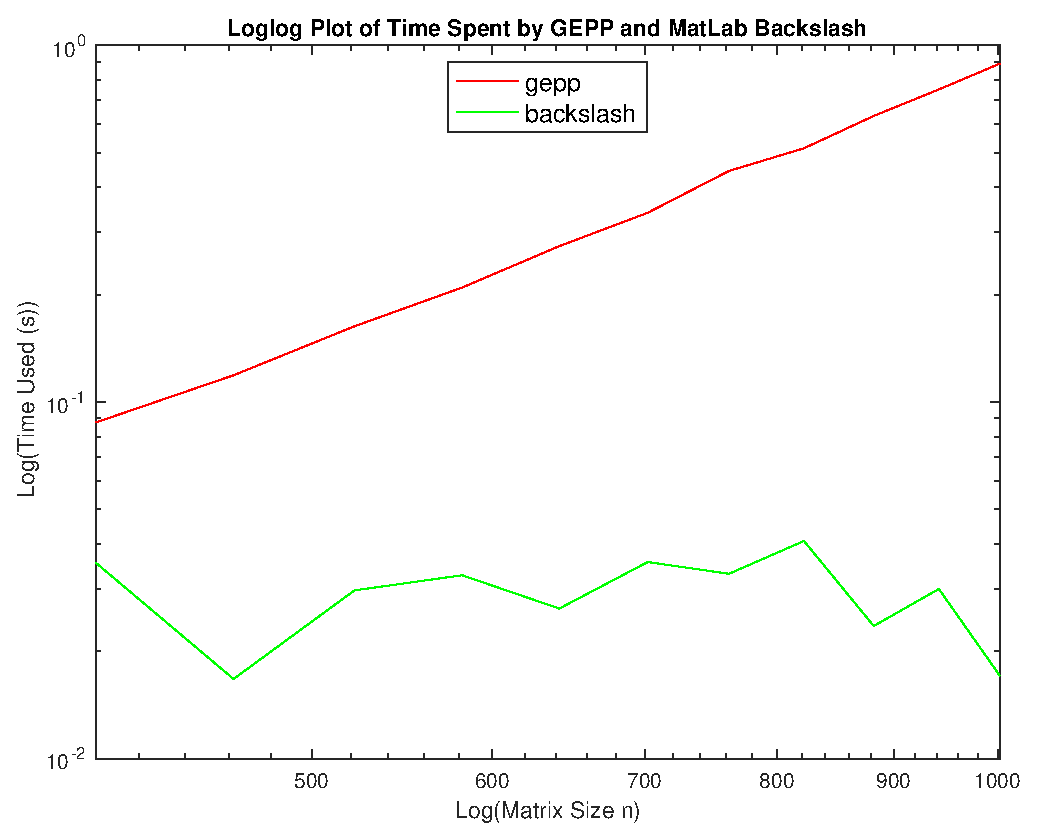
\includegraphics [width=4in]{Lab2_03.eps}
\begin{par}
Using this plot, I can fit a linear line to it. From the coefficients of this line, I can determine if the upper bound for time complexity of GEPP is satisfied. Since the coefficient of x is less than 3, the upper bound of O(n\^{}3) is satisfied. However, the reason that it might not be exactly 3 is because MatLab might have some vectorization or optimization going on in the background that enhances performance by a bit especially when the size of the matrix is large. The backslash operator is very fast compared to the GEPP routine from the textbook. In fact, for such these relatively small matrices, the slope can vary greatly and even go below 0 on some attempts, which implies that the size of the matrices being solved are way to small for the runtime to not be affected by trivial operations. The graph of backslash would likely become a more informative and increasing curve for a much larger n.
\end{par} \vspace{1em}
\begin{verbatim}
coeff_gepp = polyfit(log(n), log(times_gepp), 1);
fprintf('The equation of the line for gepp is: y = %.3fx + %.3f', ...
    coeff_gepp(1), coeff_gepp(2));

coeff_backslash = polyfit(log(n), log(times_backslash), 1);
fprintf('\nThe equation of the line for Matlab backslash is: y = %.3fx + %.3f', ...
    coeff_backslash(1), coeff_backslash(2));
\end{verbatim}

        \color{lightgray} \begin{verbatim}The equation of the line for gepp is: y = 2.562x + -17.841
The equation of the line for Matlab backslash is: y = -0.087x + -3.007\end{verbatim} \color{black}
    \begin{par}
Instead of smaller matrix sizes, I increased the interval to 1000 and started at n=2000. This allows for the loglog plot to be as smooth as possible and the resulting best-fit line has a slope of less than 3. Therefore, the time complexity of MatLab's backslash is also bounded by O(n\^{}3). This suggests that likely a similar algorithm was used with some optimization techniques that greatly improve results for relatively smaller matrices.
\end{par} \vspace{1em}
\begin{verbatim}
n=(2000:1000:12000);
times_backslash_large=zeros(11,1);
for i=1:11
    A=rand(n(i));
    b=rand(n(i),1);
    tic;
    A\b;
    times_backslash_large(i) = toc;
end

f4 = figure(4);

% plot(log(n), log(times_backslash_large), 'g')
clf(f4);
loglog(n, times_backslash_large, 'g')
hold on;
xlabel('Log(Matrix Size n)')
ylabel('Log(Time Used (s))')
title('Loglog Plot of Time Spent by MatLab Backslash')
hold off;

coeff_backslash_large = polyfit(log(n), log(times_backslash_large), 1);
fprintf('\nThe equation of the line for Matlab backslash is: y = %.3fx + %.3f', ...
    coeff_backslash_large(1), coeff_backslash_large(2));
\end{verbatim}

        \color{lightgray} \begin{verbatim}
The equation of the line for Matlab backslash is: y = 2.797x + -24.264\end{verbatim} \color{black}
    
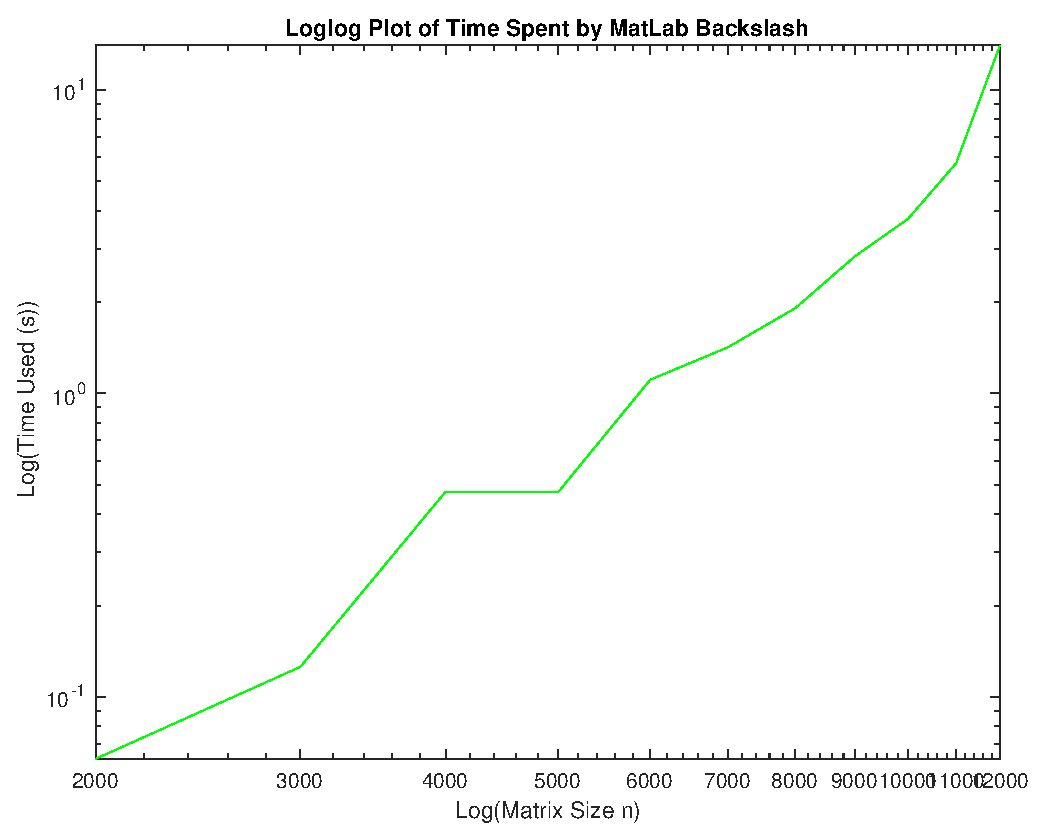
\includegraphics [width=4in]{Lab2_04.eps}



\end{document}

